\subsection{Results}
Our results broadly support the paper's central claim: adding register tokens to Vision Transformers consistently improves unsupervised object discovery performance, reduces high-norm outlier tokens, and produces cleaner attention patterns. The register improvement holds across all three model families (DINOv2, OpenCLIP, DeiT-III), all three evaluation datasets, and all qualitative experiments. However, absolute CorLoc numbers are systematically 15-20\% points below the paper's.
\subsubsection{Results reproducing original paper}
\subsubsubsection{\textbf{Object discovery: LOST quantitative evaluation.}}
This result supports the claim that registers improve unsupervised object discovery. Table~\ref{tab:object_discovery} reports our full results alongside the paper's reference numbers. The register improvement is confirmed in the correct direction for almost all six model/dataset combinations
\begin{table}[H]
\caption{CorLoc (\%) of LOST object discovery on VOC07, VOC12, and COCO datasets.}
\label{tab:object_discovery}
\begin{center}
\resizebox{35em}{!}{%
\begin{tabular}{lccc}
\toprule
\textbf{Model} & \textbf{VOC07 ours/paper} & \textbf{VOC12 ours/paper} & \textbf{COCO ours/paper}\\
\midrule
Deit-III & 19.8 / 11.7 & 21.1 / 13.1 & 20.2 / 10.7 \\
Deit-III+reg (proxy) & 21.3 / 27.1 & 22.9 / 32.7 & 23.9 / 25.1 \\
OpenCLIP & 14.2 / 38.8 & 13.1 / 44.3 & 15.3 / 31.0 \\
OpenCLIP+reg (test time proxy) & 30.5 / 37.1 & 35.6 / 42.0 & 23.3 / 27.9 \\
DINOv2 & 18.5 / 55.4 & 20.7 / 40.2 & 32.9 / 26.9 \\
DINOv2+reg & 38.4 / 55.4 & 41.6 / 60.0 & 32.9 / 42.0 \\
\bottomrule
\end{tabular}
}
\end{center}
\end{table}
\subsubsubsection{\textbf{Qualitative attention maps.}}
The qualitative attention maps (Figure~\ref{fig:qualitative_attention}) show that CLS attends broadly to the subject, while each register token produces a distinct spatial pattern. The four registers show complementary attention regions, suggesting specialisation.
\begin{figure}[ht]
\centering
    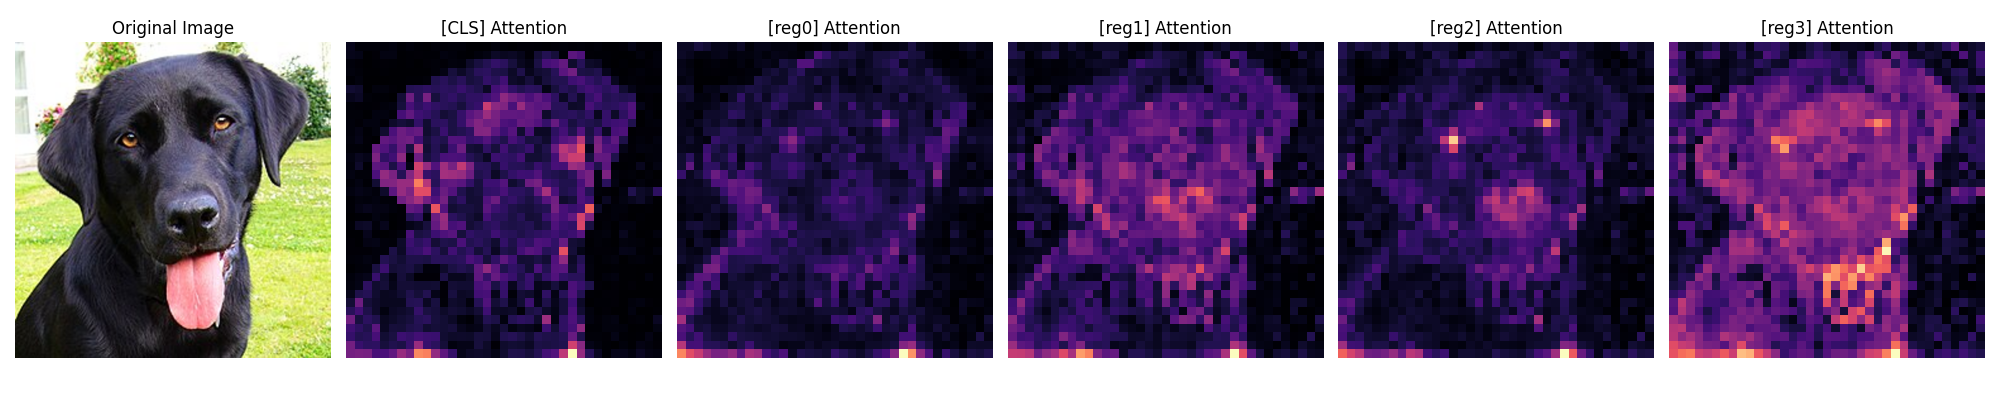
\includegraphics[width=\textwidth]{../../src/Raffo/img/dino_attention_maps_comparison.png}
\caption{Comparison of attention maps for DINOv2 of the \texttt{[CLS]} and register tokens.}
\label{fig:qualitative_attention}
\end{figure}
\subsubsubsection{\textbf{LOST intermediate maps.}} 
Figure~\ref{fig:lost_intermediate_steps} shows that for DINOv2 and DeiT-III, adding registers produces visibly cleaner dot-product and seed expansion maps — the noisy background activations present without registers are reduced. For OpenCLIP, the improvement is less striking, consistent with the paper's finding that OpenCLIP values already suppress outliers even without registers.
\begin{figure}[ht]
\centering
    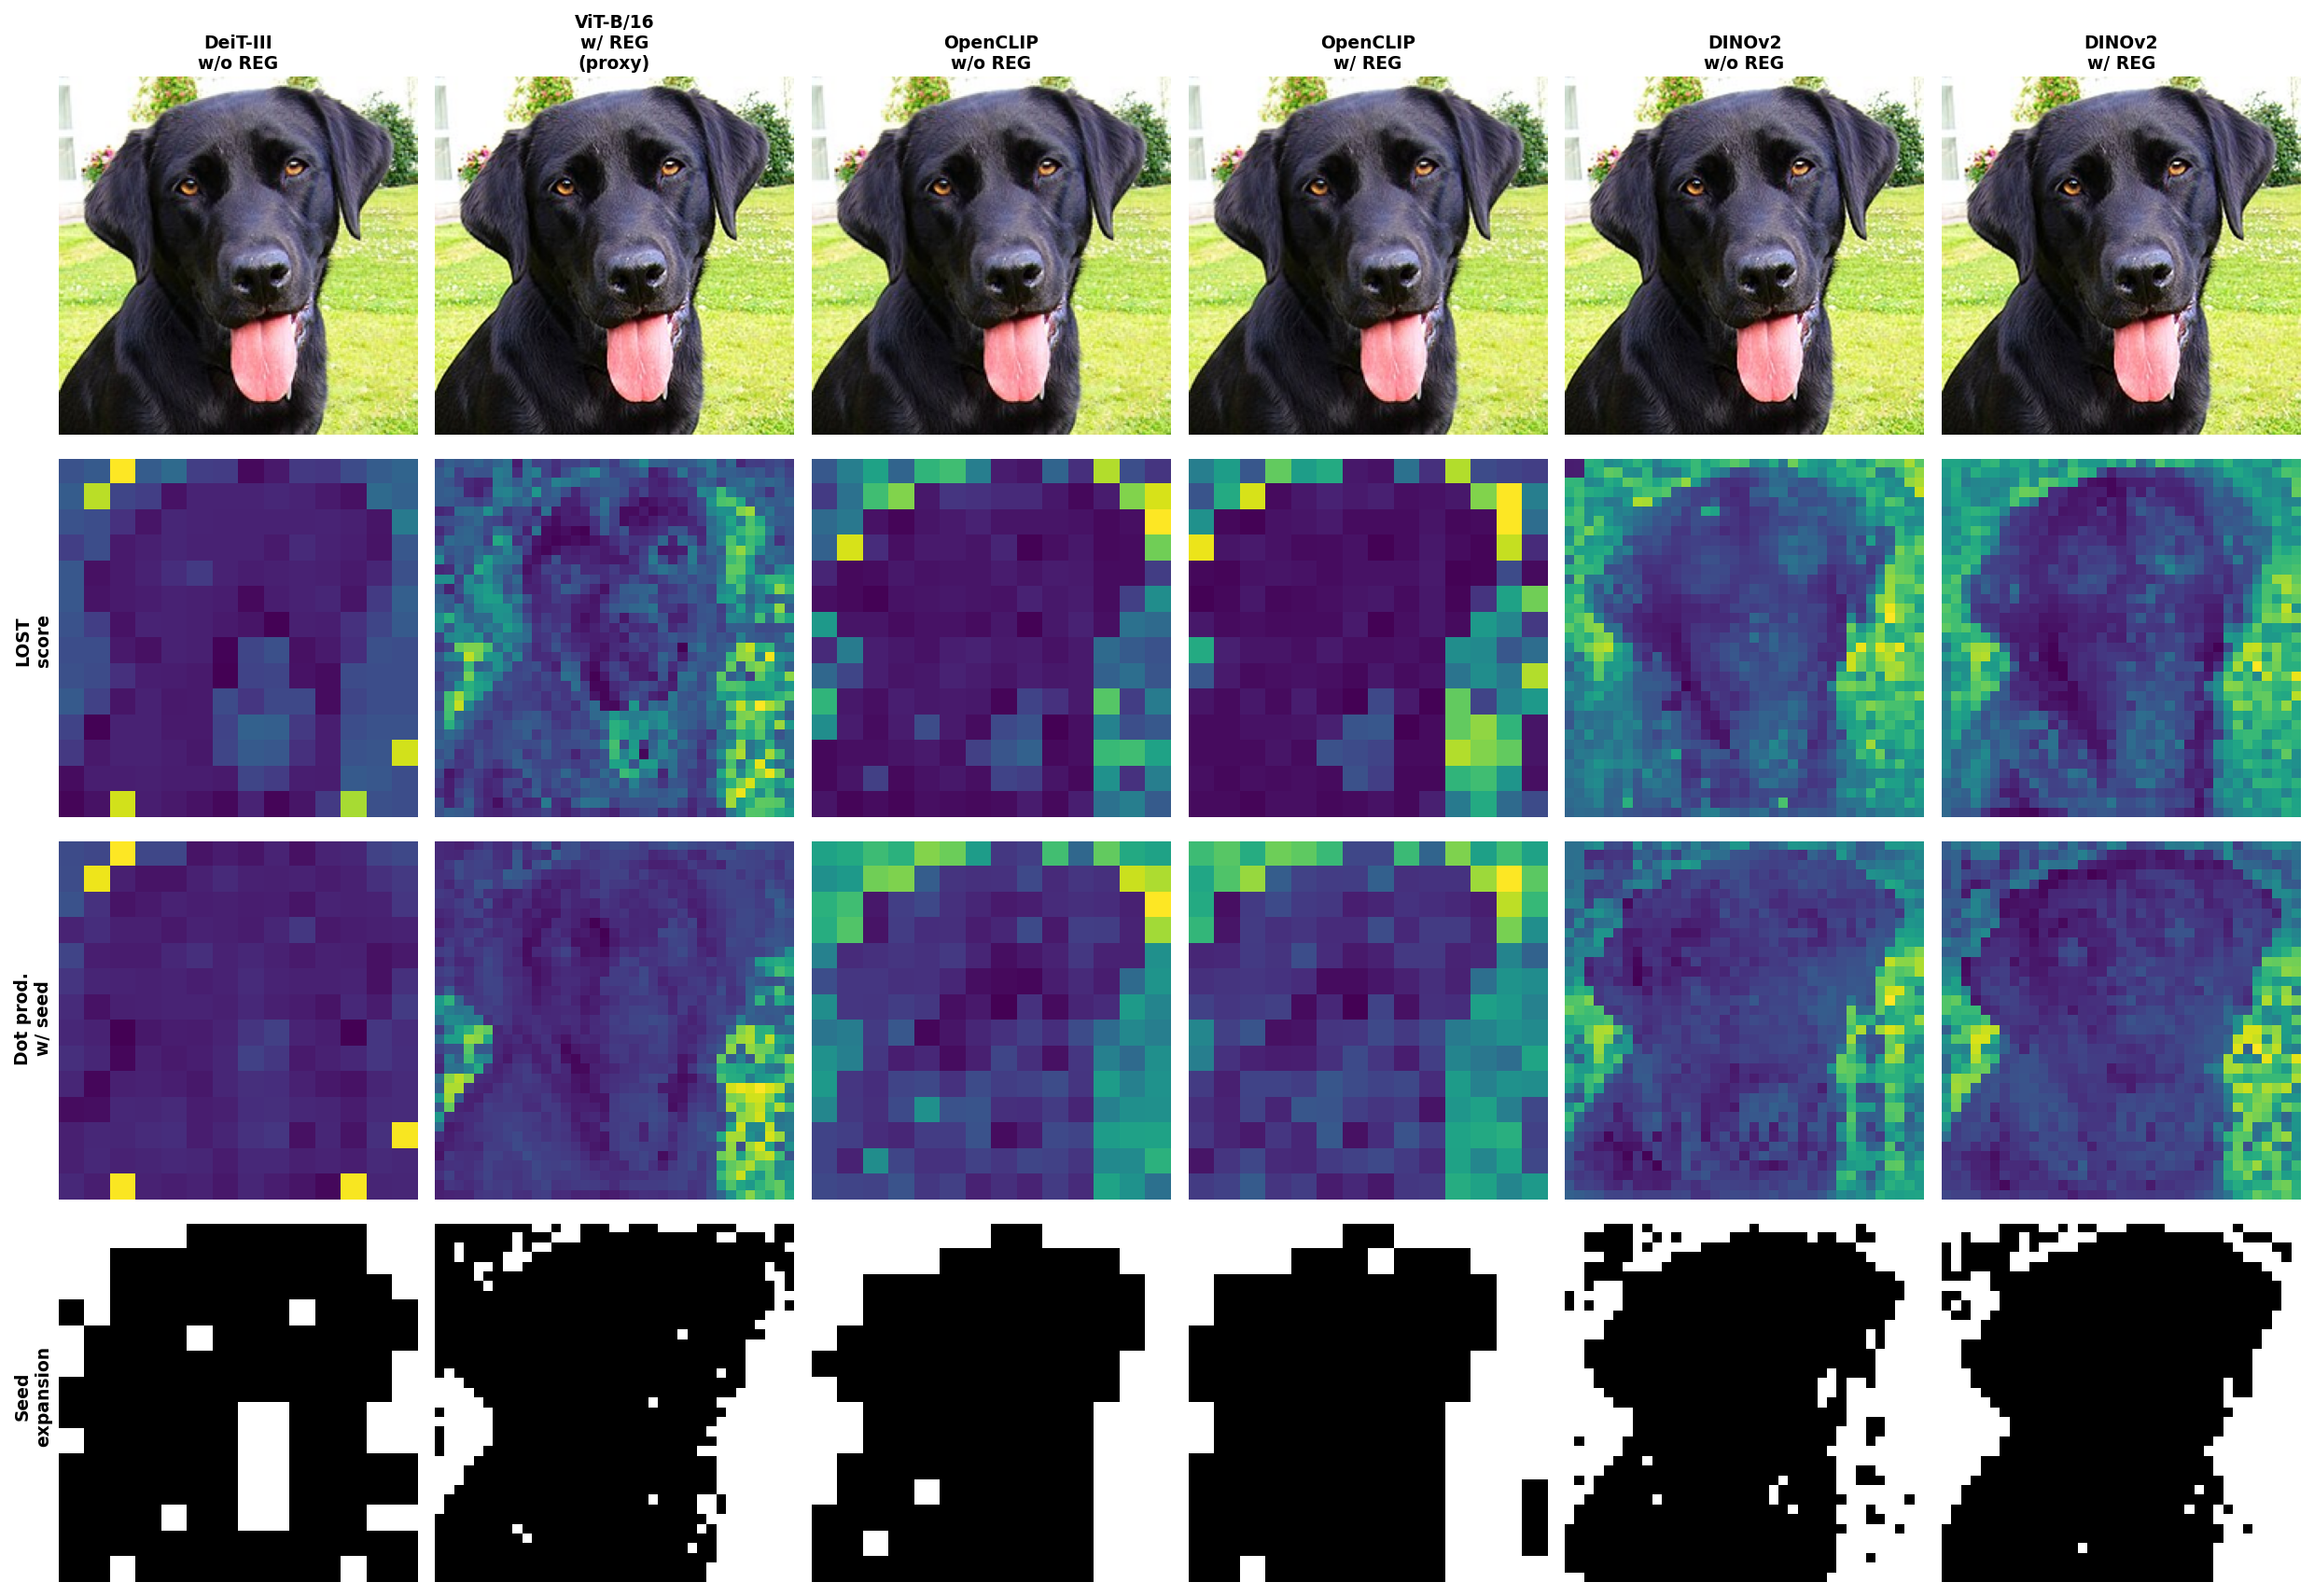
\includegraphics[width=0.8\textwidth]{../../src/Raffo/img/figure_13_replication.png}
\caption{Intermediate computations in LOST algorithm for all models. Adding registers improves the look of intermediate steps.}
\label{fig:lost_intermediate_steps}
\end{figure}
Figure~\ref{fig:seed_expansion_openclip} confirms this: the values column (right) is clean in both the no-reg and with-reg rows, which is surprising given the existence of high-norm patches in the output of OpenCLIP without registers (as shown in Figure~\ref{fig:token_norms_openclip}).
\begin{figure}[ht]
\centering
\begin{minipage}{0.65\textwidth}
    \centering
    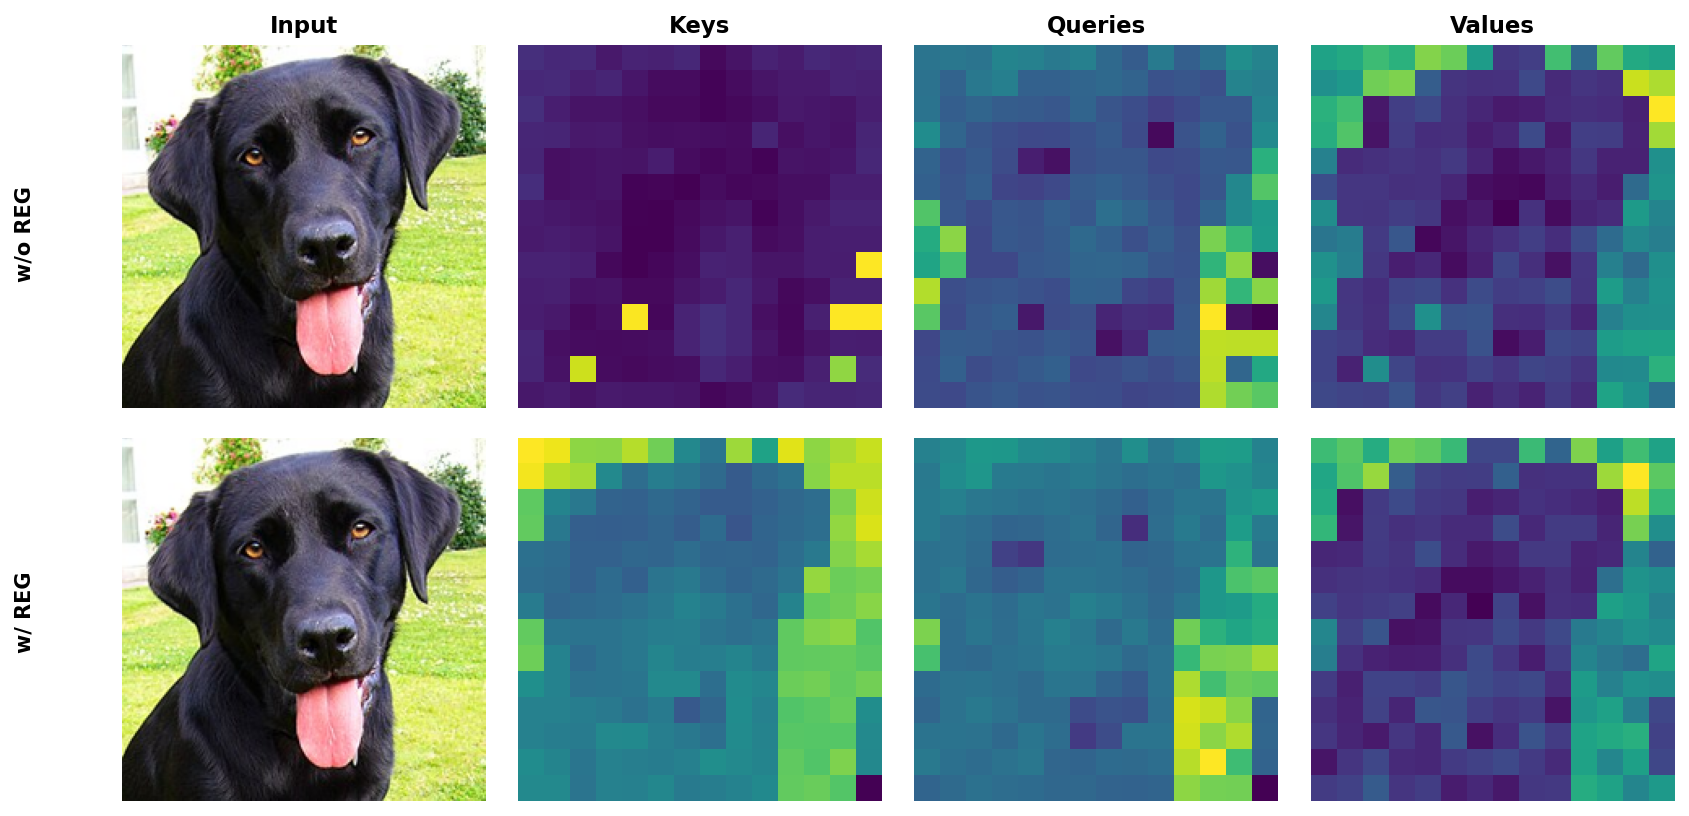
\includegraphics[width=\textwidth]{../../src/Raffo/img/figure_14_replication.png}
    \caption{Seed expansion score in LOST for OpenCLIP with and without registers for keys, queries, and values.}
    \label{fig:seed_expansion_openclip}
\end{minipage}
\hfill
\begin{minipage}{0.3\textwidth}
    \centering
    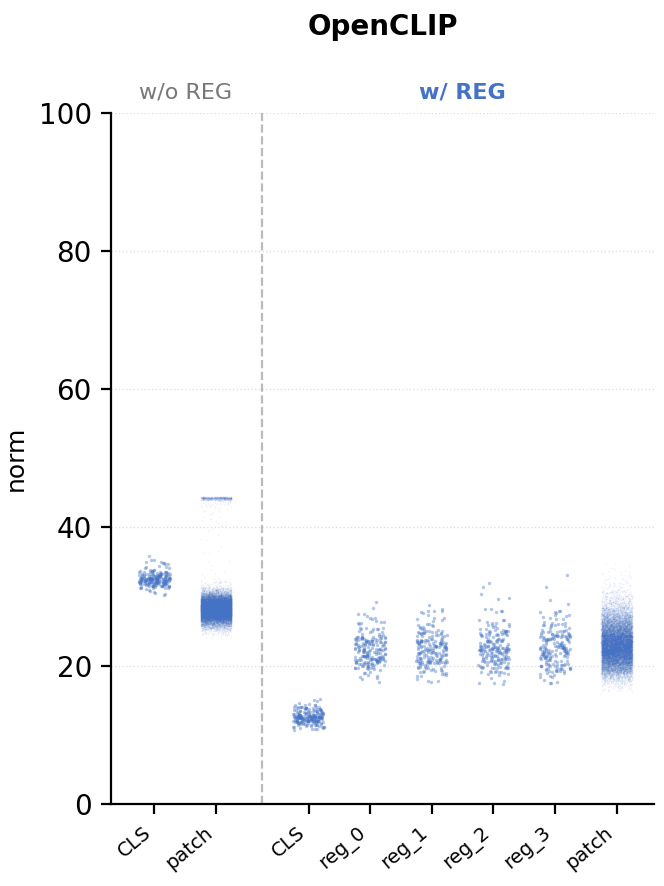
\includegraphics[width=\textwidth]{../../src/Raffo/img/figure_7_OPENCLIP.png}
    \caption{Effect of registers on the distribution of token norms for OpenCLIP.}
    \label{fig:token_norms_openclip}
\end{minipage}
\end{figure}

\subsection{\textbf{Norm distributions.}} 
\begin{figure}[ht]
\centering
    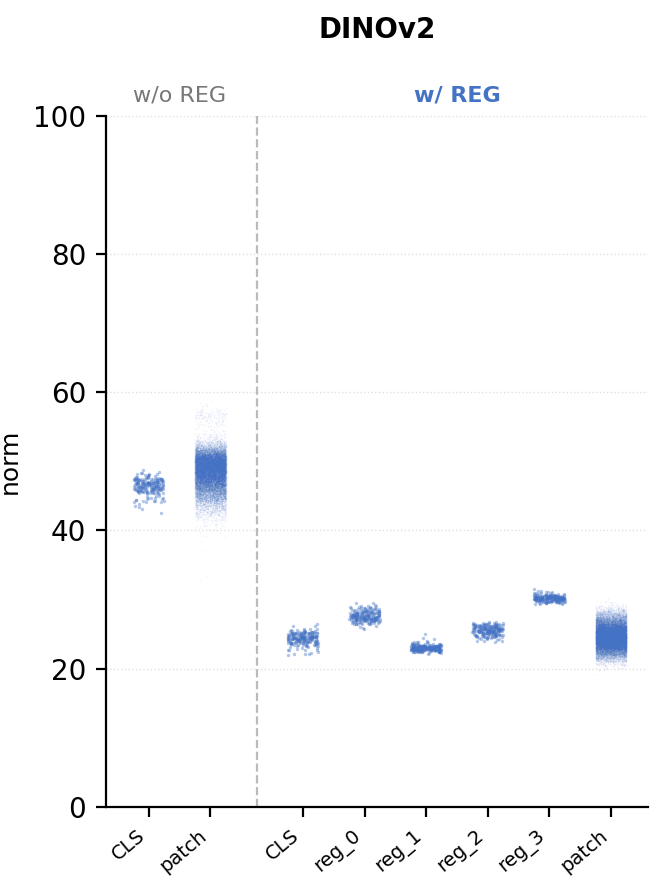
\includegraphics[width=0.3\textwidth]{../../src/Raffo/img/figure_15_replication.png}
\caption{Distribution of token norms for DINOv2 with and without registers. Registers reduce the number of high-norm outlier tokens among patch tokens.}
\label{fig:token_norms_dinov2}
\end{figure}

\subsubsection{Results beyond original paper}
Often papers don't include enough information to fully specify their experiments, so some additional experimentation may be necessary. For example, it might be the case that batch size was not specified, and so different batch sizes need to be evaluated to reproduce the original results. Include the results of any additional experiments here. Note: this won't be necessary for all reproductions.
 
\subsubsubsection{Additional Result 1}
\subsubsubsection{Additional Result 2}